% ============================================================
%  hw2_sol_numerical.tex  --  MATH 6660, Homework 2, Problems 5-7.
%  Continues the equation numbering of hw2_sol.tex (which ends at 29).
%  Build: pdflatex hw2_sol_numerical.tex   (twice)
% ============================================================
\documentclass[11pt]{article}
\usepackage[letterpaper,margin=1in]{geometry}
\usepackage[T1]{fontenc}
\usepackage{amsmath,amssymb}
\usepackage{booktabs}
\usepackage{graphicx}
\usepackage{caption}
\usepackage{enumitem}
\usepackage{bm}
\usepackage{xcolor}
\usepackage[colorlinks=true,linkcolor={blue!45!black},pdfborder={0 0 0}]{hyperref}

\newcommand{\dx}{\,\mathrm{d}x}
\newcommand{\norm}[1]{\lVert #1\rVert}
\newcommand{\Kmat}{\bm{K}}
\setlength{\parindent}{0pt}

\newcommand{\src}[1]{{\small\color{black!55}\textsf{[#1]}}}
\newcommand{\outside}[2]{%
  \par\smallskip\noindent
  \fcolorbox{red!65!black}{red!4}{%
    \parbox{0.955\linewidth}{\small
      \textbf{\color{red!65!black}NOT FROM LECTURE --- #1}\par\smallskip #2}}%
  \par\smallskip}

\newlist{steps}{itemize}{1}
\setlist[steps]{label=\textbullet, leftmargin=1.25em, topsep=3pt,
                itemsep=4pt, parsep=0pt}

\setcounter{equation}{29}      % continues hw2_sol.pdf

\begin{document}

 

\vspace{0.8em}
% ==================================================================
\section*{Problem 5}

\textbf{Problem.} For the boundary value problem with periodic boundary
conditions
\begin{align*}
  \textbf{ODE} &: \quad -\,u''+q(x)\,u=f(x),\\
  \textbf{BC1} &: \quad u(-\pi)=u(\pi),\\
  \textbf{BC2} &: \quad u'(-\pi)=u'(\pi),
\end{align*}
where $q>0$ $\forall x\in[-\pi,\pi]$:

\medskip
Numerically implement the CG(1) method on a uniform mesh with the following
functions
\[
  q(x)=3-\sin(x)-\sin(2x)-\cos(x),\quad
  f(x)=2e^{\sin(x)}e^{\cos(x)},\quad
  u(x)=e^{\sin(x)}e^{\cos(x)}.
\]
Numerically determine the convergence rate in both the \emph{energy norm} and
the $L^{2}$-norm by creating an appropriate convergence table with
\[
  M=24,49,99,199,399,799.
\]

\textbf{HINT:} You can assume a uniform grid spacing $h=2\pi/\left(M+1\right)$.
For a given $M$, you will need to write Python code that assembles the stiffness
matrix, $\underline{\underline{A}}$, and the right-hand side vector,
$\underline{b}$. I recommend that you store $\underline{\underline{A}}$ as a
sparse array using \texttt{scipy.sparse} and that you solve the resulting linear
system using the built-in conjugate gradient solver \texttt{cg} from
\texttt{scipy.sparse.linalg}. You can find documentation for how to use these
functions here: \url{https://docs.scipy.org/doc/scipy/}.

\subsection*{Verification of the data}

With $u=e^{\sin x+\cos x}$: \ $u'=u(\cos x-\sin x)$ and
$u''=u\bigl[(\cos x-\sin x)^{2}-(\sin x+\cos x)\bigr]$. Since
$(\cos x-\sin x)^{2}=1-\sin 2x$,
\begin{equation}\label{eq:p5check}
  -u''+q\,u
   =u\bigl[-1+\sin 2x+\sin x+\cos x+3-\sin x-\sin 2x-\cos x\bigr]=2u=f .
\end{equation}
Numerically $\max|-u''+qu-f|=2.7\times10^{-15}$, and
$|u(-\pi)-u(\pi)|+|u'(-\pi)-u'(\pi)|=3.3\times10^{-16}$, so $u$ satisfies both
boundary conditions.

\subsection*{Implementation }

\begin{steps}
\item Mesh and basis as in Problem 2: $N=M+1$ unknowns, $N$ elements, $h=2\pi/N$.
\item Element contributions to (16), on the reference element $[0,1]$
      with $N_0(\xi)=1-\xi$, $N_1(\xi)=\xi$:
\begin{equation}\label{eq:p5elem}
  \bm{K}^{e}_{\text{stiff}}=\frac{1}{h}\begin{bmatrix}1&-1\\-1&1\end{bmatrix},
  \qquad
  K^{e}_{ab,\,\text{mass}}=\int_{I_e}q\,N_aN_b\dx ,
  \qquad
  b^{e}_{a}=\int_{I_e}f\,N_a\dx .
\end{equation}
      The stiffness block is exact; the $q$-weighted mass block and the load are
      evaluated by $6$-point Gauss--Legendre quadrature, which is far more
      accurate than the $O(h^{2})$ discretisation error.
\item Local-to-global map, the one place periodicity enters:
\begin{equation}\label{eq:p5wrap}
  \text{element }e\ \longmapsto\ \text{nodes }\bigl(e,\ (e+1)\bmod N\bigr),
  \qquad e=0,\dots,N-1 .
\end{equation}
      The $\bmod N$ returns the last element's right node to node $0$, producing
      the corner entries $K_{0,M}=K_{M,0}$ of Problem 2. No row or column is
      deleted.
\item Solved with \texttt{scipy.sparse.linalg.cg} at tolerance $10^{-13}$,
      admissible because $\Kmat$ is symmetric positive definite (Problem 2).
\item Both error norms are computed element by element with the same Gauss rule,
      using $u'$ analytically and $U'$ constant on each element.
\end{steps}

\subsection*{Convergence table}

Observed rate between consecutive meshes:
\begin{equation}\label{eq:p5rate}
  r_k=\frac{\ln\bigl(E_{k-1}/E_k\bigr)}{\ln\bigl(h_{k-1}/h_k\bigr)} .
\end{equation}

\begin{center}
\begin{tabular}{rccccc}
\toprule
$M$ & $h$ & $\|u-U\|_{L^2}$ & rate & $\|u-U\|_E$ & rate\\
\midrule
24 & 2.5133e-01 & 2.7134e-02 & --- & 4.1346e-01 & ---\\
49 & 1.2566e-01 & 6.7860e-03 & 2.00 & 2.0691e-01 & 1.00\\
99 & 6.2832e-02 & 1.6967e-03 & 2.00 & 1.0348e-01 & 1.00\\
199 & 3.1416e-02 & 4.2418e-04 & 2.00 & 5.1743e-02 & 1.00\\
399 & 1.5708e-02 & 1.0605e-04 & 2.00 & 2.5872e-02 & 1.00\\
799 & 7.8540e-03 & 2.6511e-05 & 2.00 & 1.2936e-02 & 1.00\\
\bottomrule
\end{tabular}

\end{center}

\subsection*{Conclusion}

\[
  \norm{u-U}_{E}=O(h^{1.00}),
  \qquad
  \norm{u-U}_{L^{2}}=O(h^{2.00}),
\]
confirming (22) (first order in the energy norm) and
(29) (second order in $L^{2}$).

\begin{figure}[htbp]
\centering
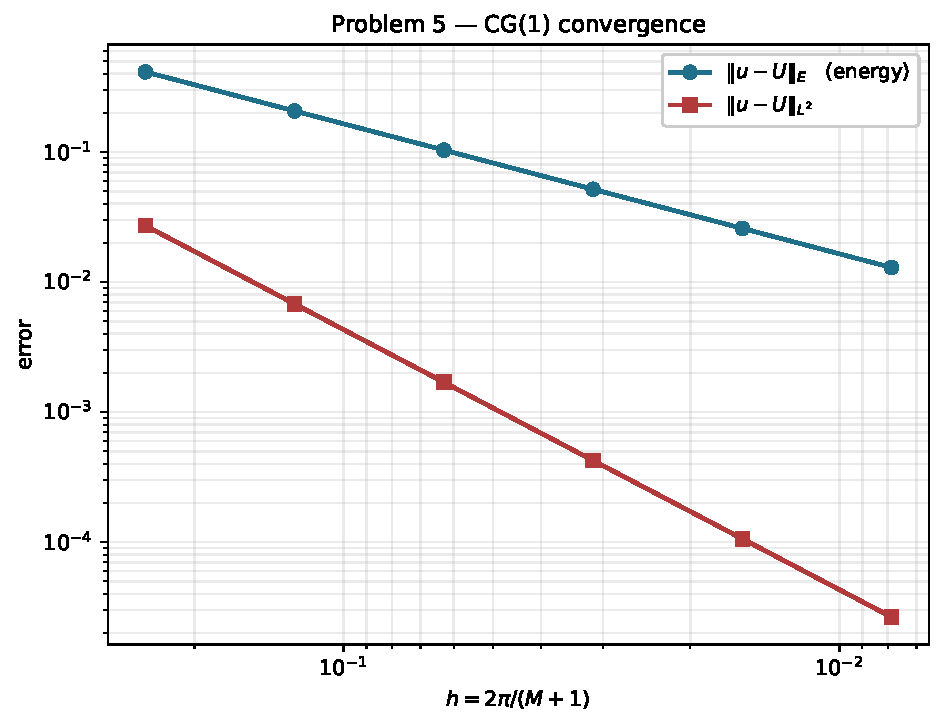
\includegraphics[width=0.80\linewidth]{hw2_p5_convergence.pdf}
\caption{Problem 5. CG(1) convergence for the periodic problem: energy-norm and
$L^{2}$-norm errors against the mesh size $h=2\pi/(M+1)$, for
$M=24,49,99,199,399,799$. Both curves are straight on log--log axes, with
measured slopes $1.00$ and $2.00$.}

\end{figure}

\clearpage
\begin{figure}[htbp]
\centering
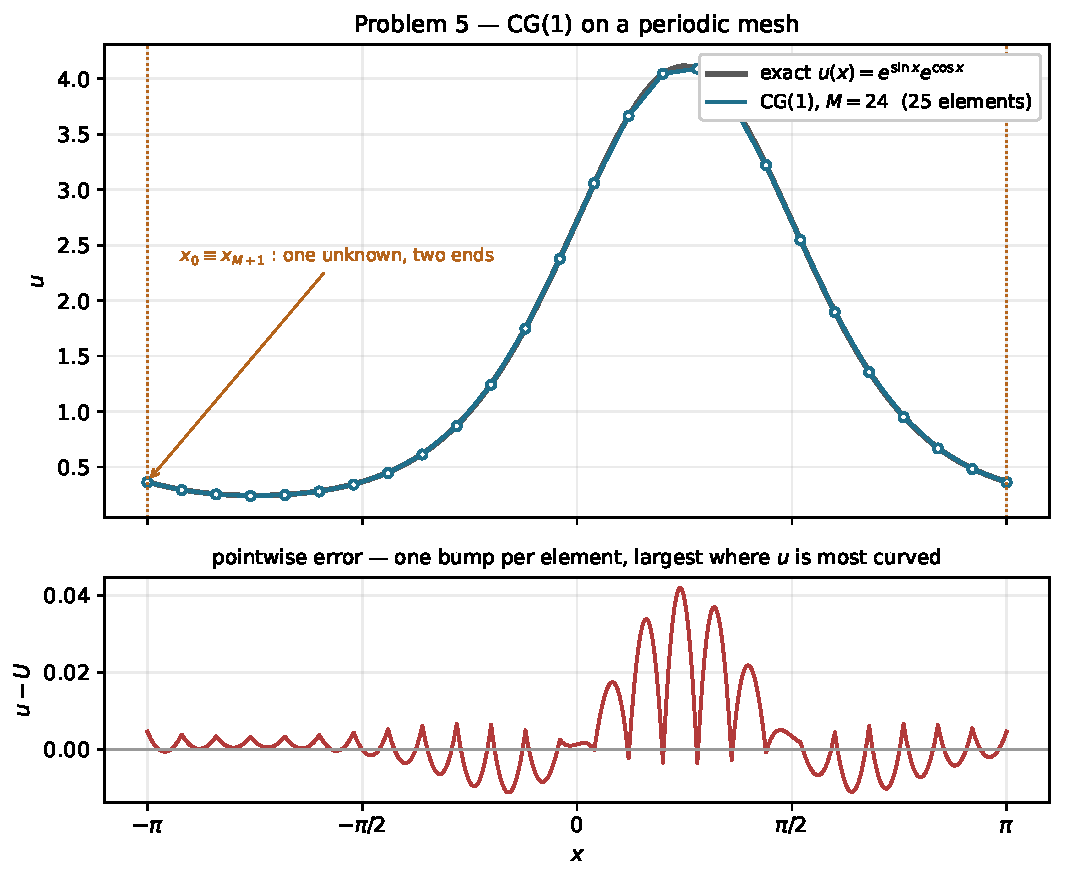
\includegraphics[width=0.92\linewidth]{hw2_p5_solution.pdf}
\caption{Problem 5. \textbf{Top:} exact solution and the CG(1) solution at
$M=24$; the circles are the $25$ nodes, and the dotted lines at $x=\pm\pi$ mark
the same point of the domain, one unknown $\xi_0$ serving both ends.
\textbf{Bottom:} the pointwise error $u-U$, one bump per element and largest
where $u$ is most strongly curved.}
\end{figure}

\clearpage
% ==================================================================
\section*{Problem 6}

\textbf{Problem.} Implement the CG(2) method (piecewise quadratics) as discussed
in class for $-u''=f$ on $(0,1)$, $u(0)=u(1)=0$.

 

\subsection*{Mesh and numbering  }

\begin{steps}
\item $h=1/(M+1)$, $M+1$ elements, nodes indexed by half-integers:
\begin{equation}\label{eq:p6num}
  x_{k/2}=\tfrac{kh}{2},\quad k=0,1,\dots,2M+2:
  \qquad k\ \text{even}\Rightarrow\text{vertex},
  \qquad k\ \text{odd}\Rightarrow\text{midside}.
\end{equation}
\item $2M+3$ nodes; the two Dirichlet ends $k=0$ and $k=2M+2$ are eliminated,
      leaving $2M+1$ unknowns --- the size Lecture 10 gives.
\end{steps}

\subsection*{Basis and element stiffness }

\begin{steps}
\item On the reference element $[0,1]$:
\begin{equation}\label{eq:p6shape}
  N_0(\xi)=2\bigl(\xi-\tfrac12\bigr)(\xi-1),\qquad
  N_1(\xi)=4\xi(1-\xi),\qquad
  N_2(\xi)=2\xi\bigl(\xi-\tfrac12\bigr),
\end{equation}
      equal to $1$ at $\xi=0,\tfrac12,1$ respectively and $0$ at the other two.
\item With $\mathrm{d}N_a/\mathrm{d}x=h^{-1}\mathrm{d}N_a/\mathrm{d}\xi$ and
      $\mathrm{d}N_0/\mathrm{d}\xi=4\xi-3$, $\mathrm{d}N_1/\mathrm{d}\xi=4-8\xi$,
      $\mathrm{d}N_2/\mathrm{d}\xi=4\xi-1$, the element stiffness integrates
      exactly to
\begin{equation}\label{eq:p6Ke}
  \bm{K}^{e}=\frac{1}{3h}
  \begin{bmatrix} 7&-8&1\\ -8&16&-8\\ 1&-8&7\end{bmatrix}
  \qquad\text{(ordering: vertex, midside, vertex).}
\end{equation}
\end{steps}

\subsection*{Load vector  }

\begin{steps}
\item Assembled from the exact $P_2$ element mass matrix applied to nodal $f$:
\begin{equation}\label{eq:p6load}
  \bm{b}^{e}=h\,\bm{M}^{e}\bm{f}^{e},
  \qquad
  \bm{M}^{e}=\frac{1}{30}
  \begin{bmatrix}4&2&-1\\ 2&16&2\\ -1&2&4\end{bmatrix},
  \qquad
  \bm{f}^{e}=\bigl(f(x_{j-1}),\,f(x_{j-1/2}),\,f(x_j)\bigr)^{T},
\end{equation}
      which reproduces the two lecture stencils row by row.
\item Exact quadrature of $\int f N_a\dx$ was also implemented as a check; it
      changes the asymptotic rates not at all, and the table entries only in the
      third digit at $M=24$ and $49$.
\end{steps}

\subsection*{Verification against Lecture 10}

Assembling \eqref{eq:p6Ke} and striking out the two Dirichlet rows and columns,
the code prints $3h\Kmat$ for $M=4$ (a $9\times9$ system):
\begin{equation}\label{eq:p6assembled}
  3h\,\Kmat=
  \setlength{\arraycolsep}{3.2pt}
  \renewcommand{\arraystretch}{0.92}
  \begin{bmatrix}
   16 & -8 &    &    &    &    &    &    &   \\
   -8 & 14 & -8 &  1 &    &    &    &    &   \\
      & -8 & 16 & -8 &    &    &    &    &   \\
      &  1 & -8 & 14 & -8 &  1 &    &    &   \\
      &    &    & -8 & 16 & -8 &    &    &   \\
      &    &    &  1 & -8 & 14 & -8 &  1 &   \\
      &    &    &    &    & -8 & 16 & -8 &   \\
      &    &    &    &    &  1 & -8 & 14 & -8\\
      &    &    &    &    &    &    & -8 & 16
  \end{bmatrix}
\end{equation}
This reproduces Lecture 10 exactly: $16/3h$ on the midside diagonal, $14/3h$ on
the vertex diagonal, $-8/3h$ on the first off-diagonal, $1/3h$ two places out
from a vertex row. The matrix is symmetric positive definite, so \texttt{cg}
applies; its pattern is pentadiagonal rather than tridiagonal.

\clearpage
% ==================================================================
\section*{Problem 7}

\textbf{Problem.} Apply the method to
\[
  u(x)=e^{1-\cos(2\pi x)-\sin(2\pi x)}-1,\qquad
  f(x)=4\pi^{2}e^{1-\cos(2\pi x)-\sin(2\pi x)}
       \bigl[\sin(4\pi x)-\cos(2\pi x)-\sin(2\pi x)-1\bigr],
\]
and determine the convergence rate in both norms for
$M=24,49,99,199,399,799$.

\subsection*{Verification of the data}

Write $g=1-\cos 2\pi x-\sin 2\pi x$, so $u=e^{g}-1$ and
\[
  g'=2\pi(\sin 2\pi x-\cos 2\pi x),\qquad
  g''=4\pi^{2}(\cos 2\pi x+\sin 2\pi x),\qquad
  (g')^{2}=4\pi^{2}(1-\sin 4\pi x).
\]
Then $u''=e^{g}\bigl[(g')^{2}+g''\bigr]$, so
\begin{equation}\label{eq:p7check}
  -u''=4\pi^{2}e^{g}\bigl[\sin 4\pi x-\cos 2\pi x-\sin 2\pi x-1\bigr]=f ,
\end{equation}
and $u(0)=u(1)=e^{0}-1=0$. Numerically $\max|-u''-f|=3.4\times10^{-13}$ and
$|u(0)|+|u(1)|=2.2\times10^{-16}$.

\subsection*{Convergence table}

\begin{center}
\begin{tabular}{rccccc}
\toprule
$M$ & $h$ & $\|u-U\|_{L^2}$ & rate & $\|u-U\|_E$ & rate\\
\midrule
24 & 4.0000e-02 & 1.1386e-03 & --- & 1.8042e-01 & ---\\
49 & 2.0000e-02 & 1.4056e-04 & 3.02 & 4.5288e-02 & 1.99\\
99 & 1.0000e-02 & 1.7513e-05 & 3.00 & 1.1334e-02 & 2.00\\
199 & 5.0000e-03 & 2.1874e-06 & 3.00 & 2.8341e-03 & 2.00\\
399 & 2.5000e-03 & 2.7336e-07 & 3.00 & 7.0857e-04 & 2.00\\
799 & 1.2500e-03 & 3.4169e-08 & 3.00 & 1.7715e-04 & 2.00\\
\bottomrule
\end{tabular}

\end{center}

\subsection*{Conclusion}

\[
  \norm{u-U}_{E}=O(h^{2.00}),
  \qquad
  \norm{u-U}_{L^{2}}=O(h^{3.00}),
\]
matching the CG(2) estimates of Lecture 10,
$\norm{u-U}_{E}\le c\norm{h^{2}u'''}$ and $\norm{u-U}\le c\norm{h^{3}u'''}$.
Each additional polynomial degree buys one power of $h$ in both norms, and the
$L^{2}$ rate remains one order ahead of the energy rate.

\begin{figure}[htbp]
\centering
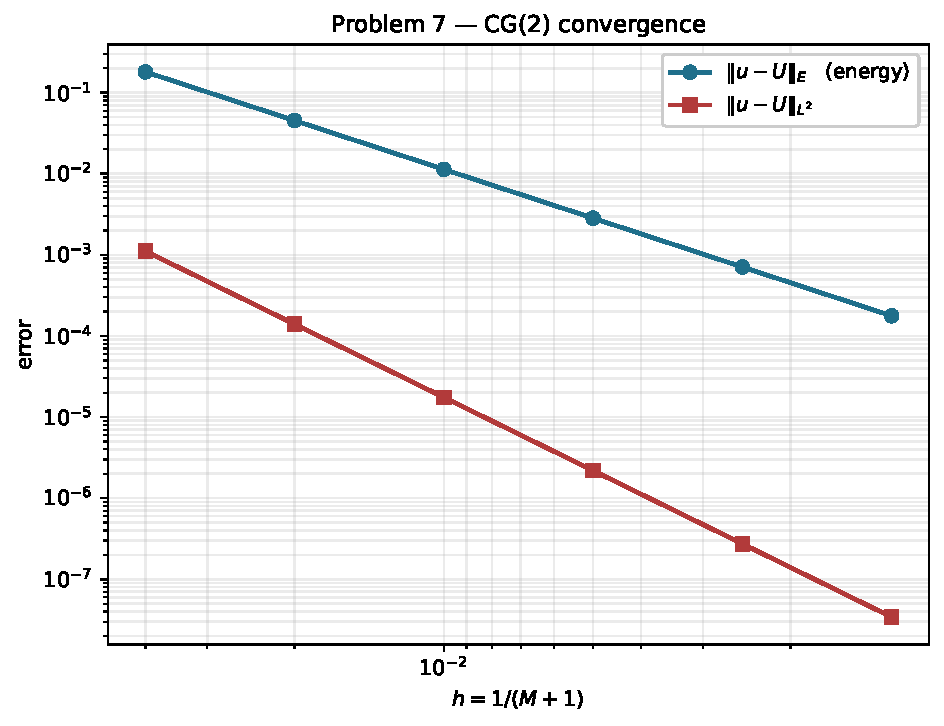
\includegraphics[width=0.80\linewidth]{hw2_p67_convergence.pdf}
\caption{Problem 7. CG(2) convergence: energy-norm and $L^{2}$-norm errors
against the mesh size $h=1/(M+1)$, for $M=24,49,99,199,399,799$. Measured
slopes $2.00$ and $3.00$.}

\end{figure}

\clearpage
\begin{figure}[htbp]
\centering
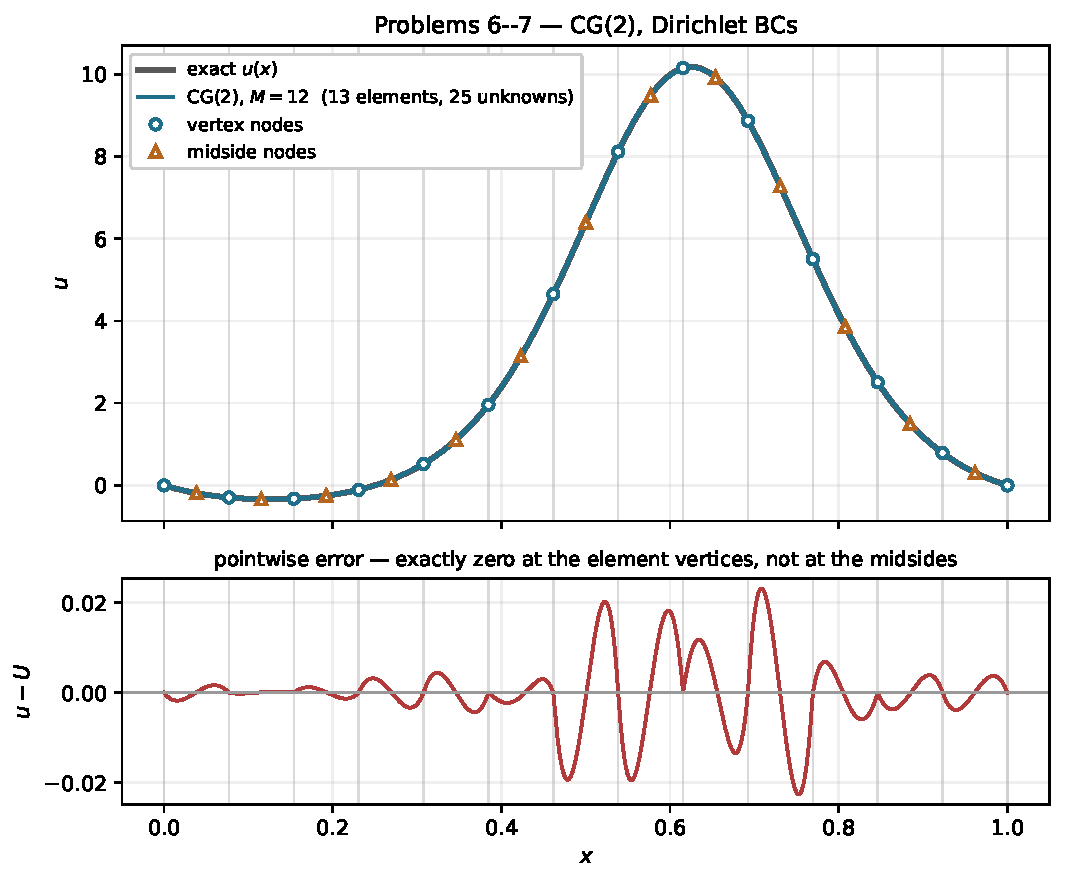
\includegraphics[width=0.92\linewidth]{hw2_p67_solution.pdf}
\caption{Problem 7. \textbf{Top:} exact solution and the CG(2) solution at
$M=12$; circles are vertex nodes and triangles midside nodes.
\textbf{Bottom:} the pointwise error $u-U$.}
\end{figure}

\end{document}
